\subsection{Long-slit spectroscopy, LM band}
\label{ssec:recipes_lss_lm}

A draft of the reduction cascade is shown in
Fig.~\ref{Fig:LMLssAssomap} together with the data processing table
(Table~\ref{Tab:LssDatProc}). The first part concerns the detector
calibrations, which are independent of the observing mode and already
described in Section~6.1 in \cite{DRLS}. This affects the
dark correction, linearity and gain determination and bad pixel
detection. The second step is the flatfielding, followed by the wavelength
correction and the determination of the response curve for the flux calibration. Subsequently, the main reduction is conducted, which applies
the previously created master calibration files to the science frames. Finally, the telluric absorption correction is applied using the modelling approach with \texttt{molecfit}. 

Special emphasis has to be drawn to the effects of the Earth's
atmosphere in several respects:
\begin{itemize}
\item Wavelength calibration: Absorption/emission features are to be
  used for the wavelength calibration. Thus, a good knowledge on (
  identification of these features is crucial for the accuracy of the
  wavelength calibration.
\item Telluric correction: In the MIR regime telluric absorption is
  one of the most dominant effects visible in spectra. Modelling
  approaches like \texttt{molecfit} heavily rely on accurate
  atmospheric input profiles, which represent the actual state and
  composition of the Earth's atmosphere. This especially applies to
  the \ac{PWV} content since this is the most
  dominant and most variable species.
\item Atmospheric dispersion: \ac{METIS} will have \ac{ADC}s compensating the
  effect of atmospheric dispersion. However, for technical reasons
  these ADCs are fixed at several positions. This means that the
  compensation is only partially. This leads to two practical effects:
  (a) wavelength-dependent slit losses and (b) distortions in both,
  the spatial and the spectral direction (see \cite{METIS-ADC_study}
  for more details). For both, the pipeline needs to correct
  for. Since airmass, ambient temperature/pressure, slit orientation,
  and the properties of the \ac{ADC}s are known, the only required
  parameter to be determined for the compensation is the \ac{PWV}.
\end{itemize}
It is therefore crucial to have a radiometer (e.g.\ L-HATPRO)
available at the \ac{ELT}, which provides direct measurements of the \ac{PWV}
along the observation direction.

As the flux standard stars are treated very similar to the science
data, we also included them in this recipe. For the observatory
pipeline at the mountain, this recipe most probably has to be split
into dedicated recipes for processing flux standards and a science
data, since the observing templates directly trigger the corresponding
recipes after their execution.

\subsection{\REC{metis_LM_lss_wave}:}
This recipe aims at deriving the wavelength solution on basis of the sky lines visible in the science data. In a first step, the detector signature is removed by applying the master calibration files derived in the previous steps, following by the background subtraction and the application of the RSRF. The distortion of the lines (i.e. possible tilt, curvature,...) and the wavelength solution is determined by the algorithm described in Sect.\,8.5 in \cite{DRLS}.

% \begin{figure}[ht]
%   \centering
%   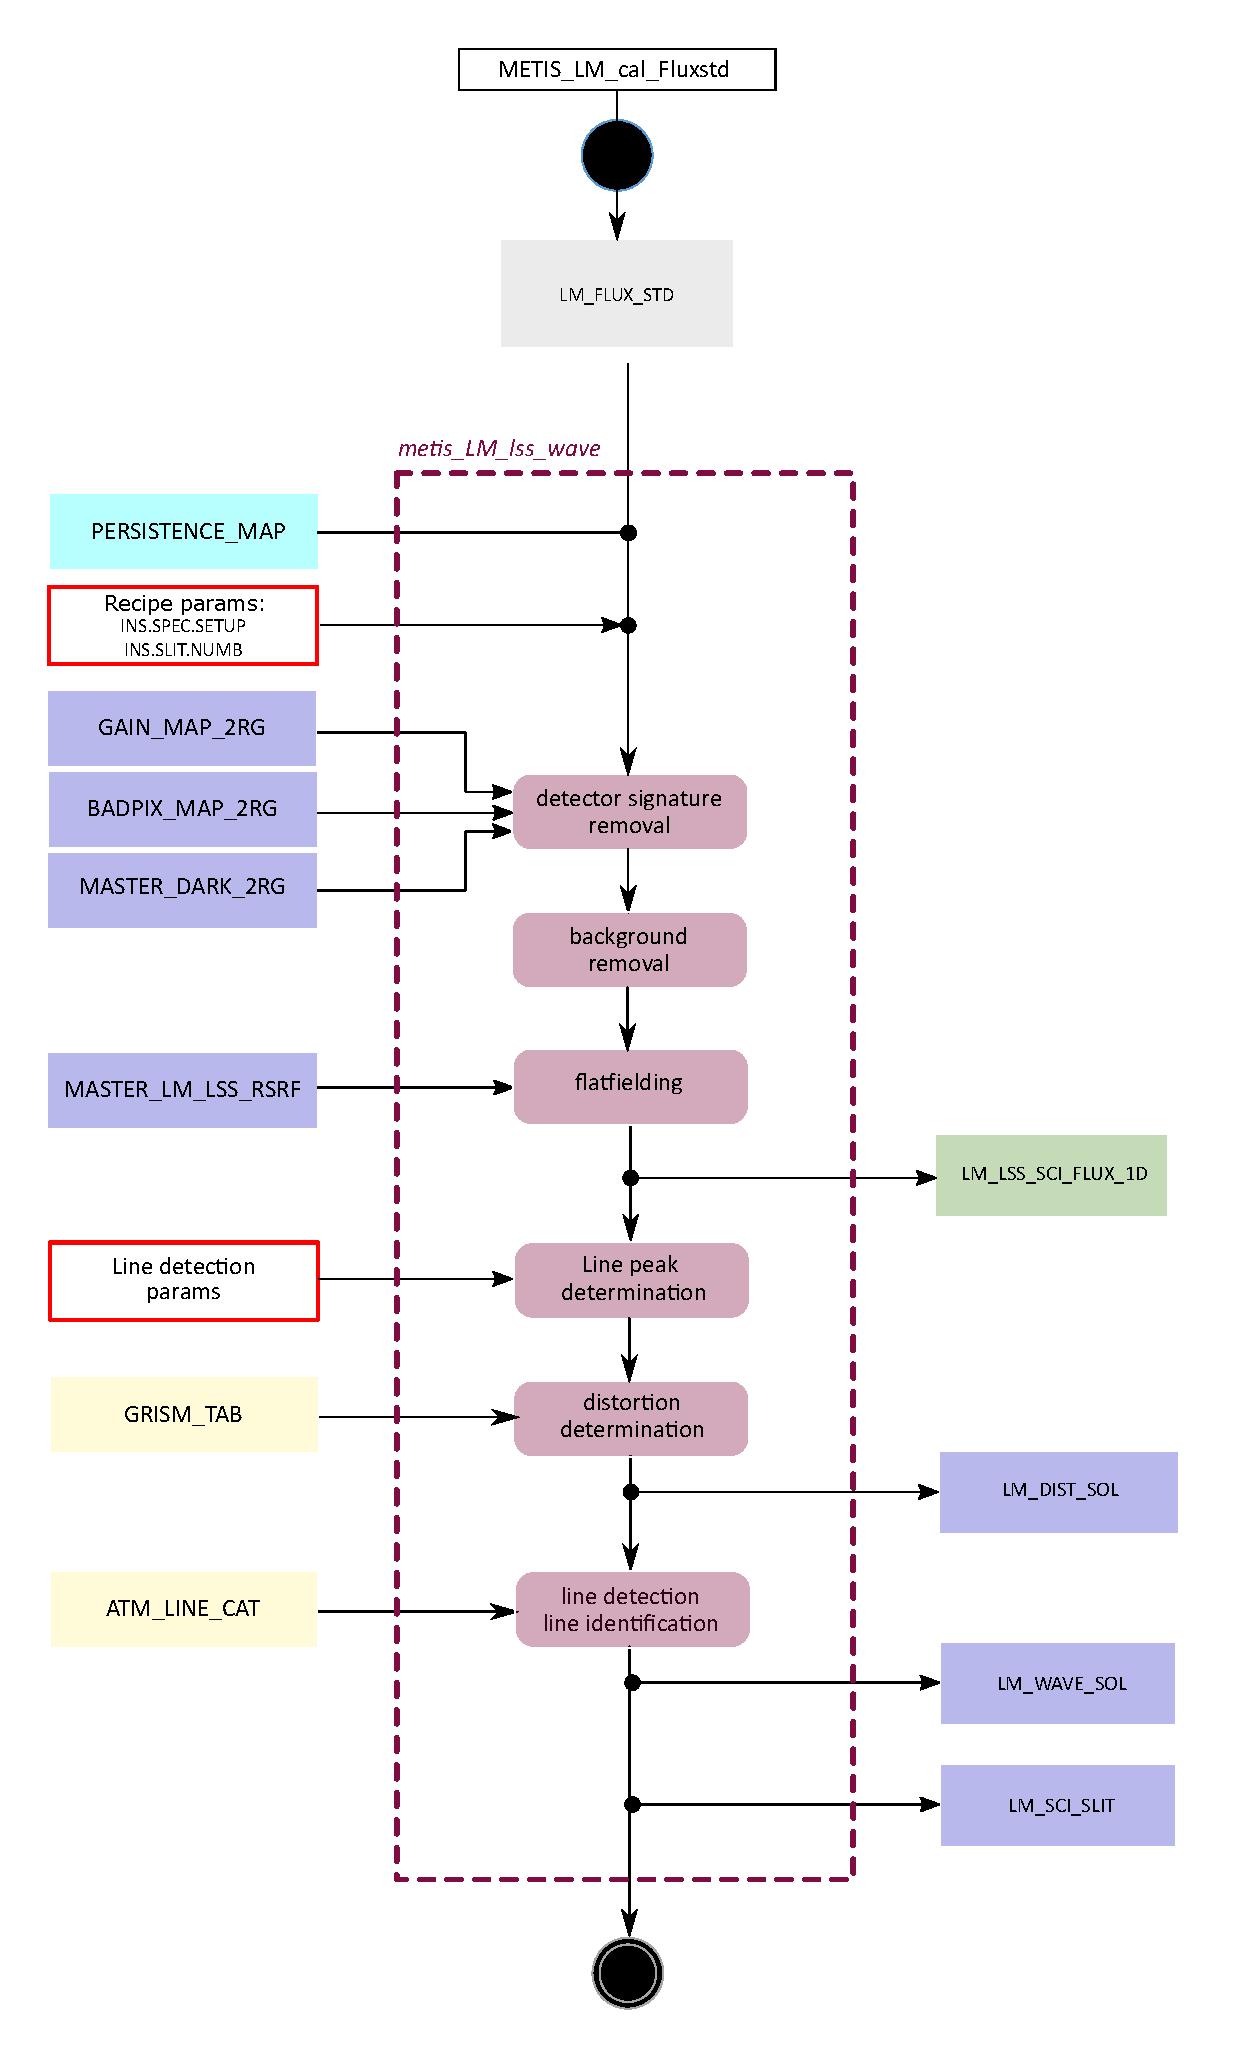
\includegraphics[width=0.5\textheight]{figures/metis_lm_lss_wave_0.62.pdf}
%   \caption[Recipe for the LM-LSS mode wavelength calibration]{Recipe for the LM-LSS mode wavelength calibration.  }
%   \label{Fig:rec_lm_lss_wave}
% \end{figure}
\begin{figure}[ht]
  \centering
  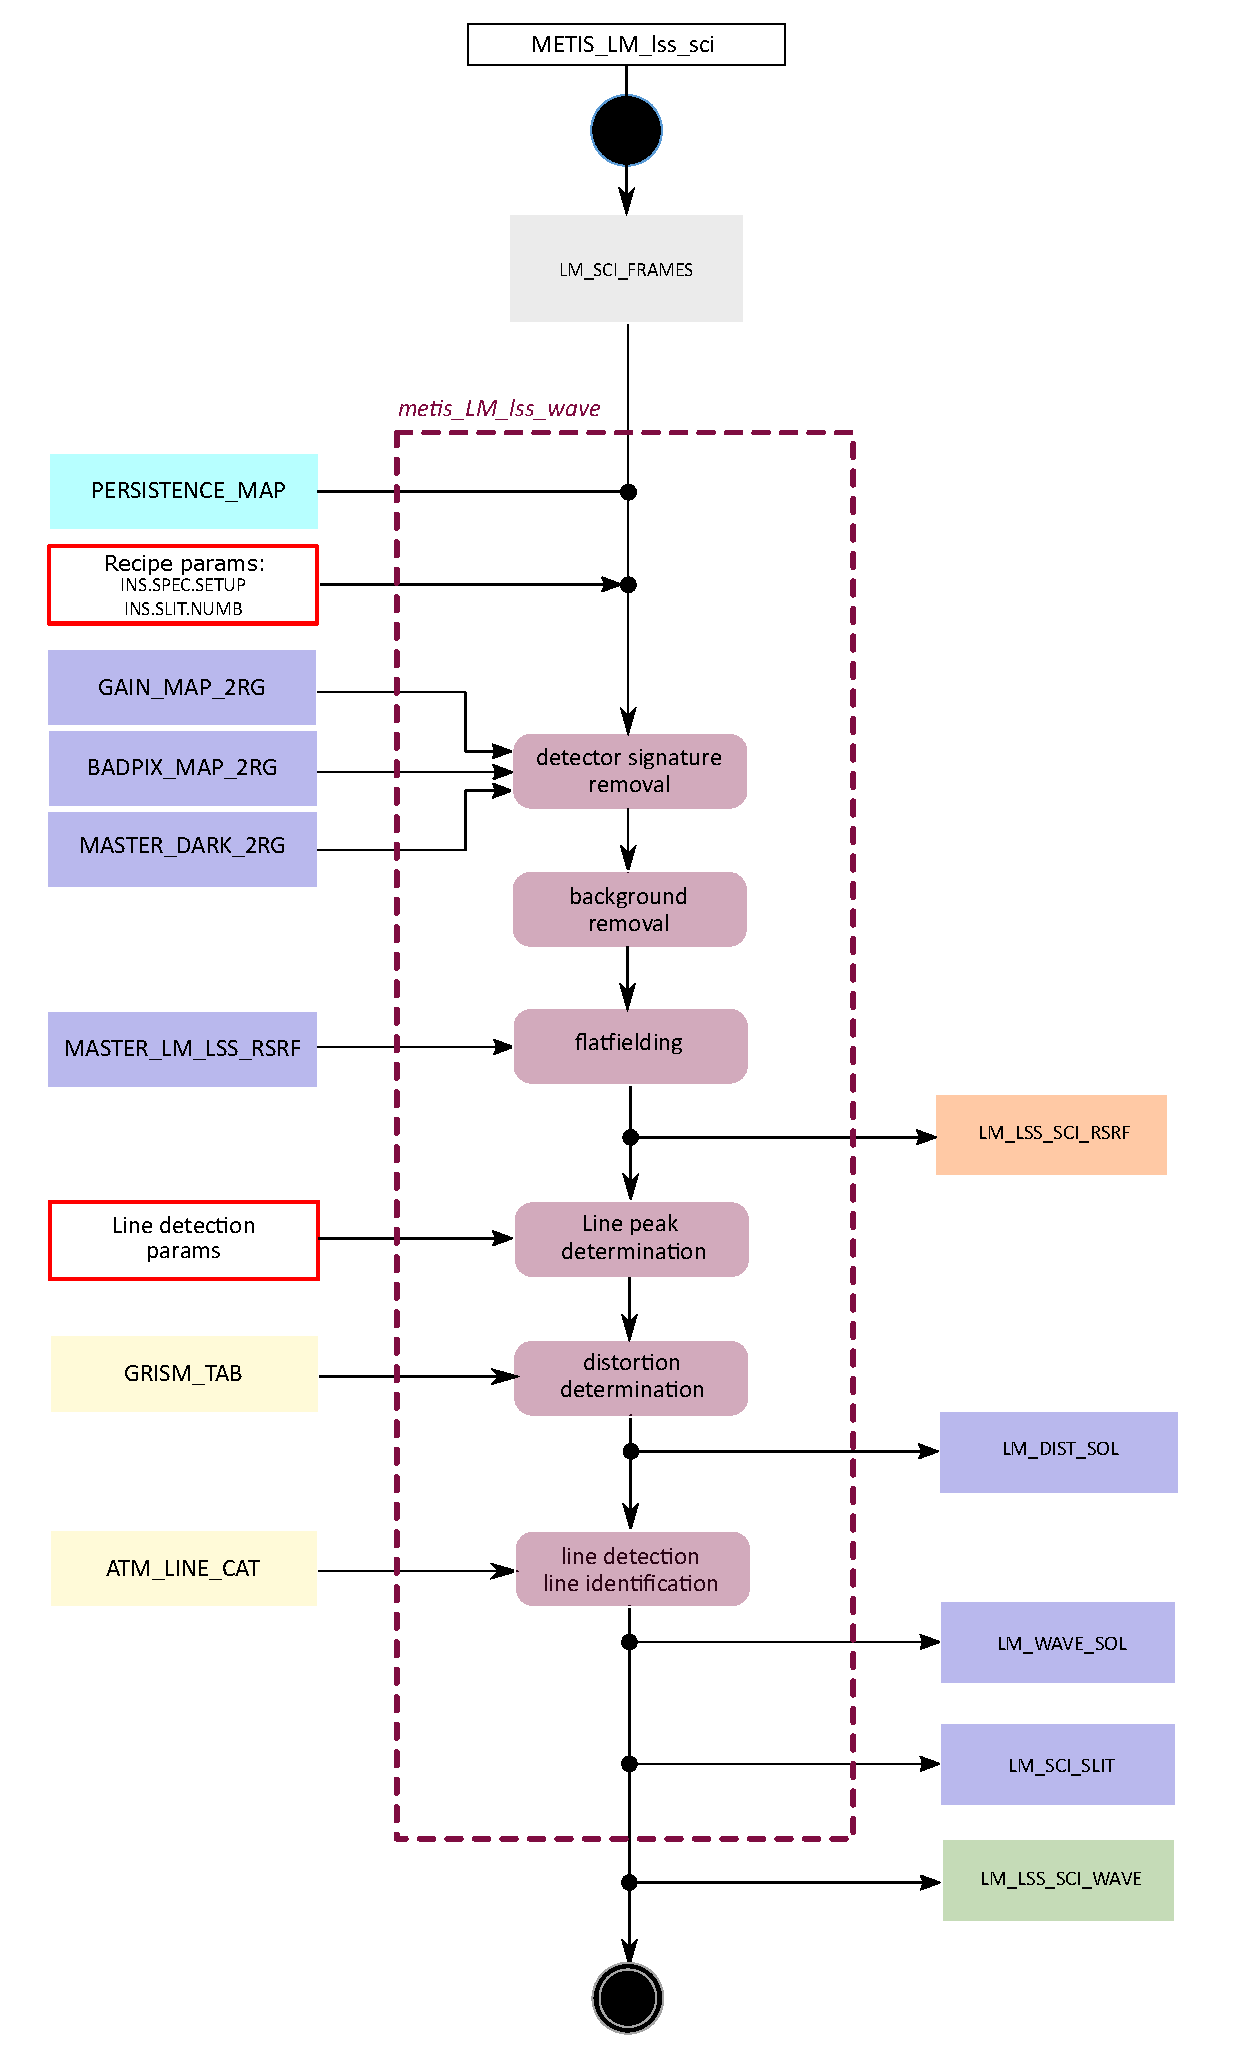
\includegraphics[width=0.5\textheight]{figures/metis_lm_lss_wave_v0.64.pdf}
  \caption[Recipe: \REC{metis_LM_lss_wave}]{\REC{metis_LM_lss_wave} --
    Creation of the LM LSS master wavelength correction.}
  \label{Fig:rec_lm_lss_wave}
\end{figure}
\clearpage

\begin{recipedef}
Name:		& \REC{metis_LM_lss_wave} \\
Purpose:	& Wavelength calibration \\
Type:		& Calibration\\
Requirements: & METIS-6084, METIS-1371, METIS-6074 \\
Observing templates: & \TPL{METIS_spec_lm_acq}, \\
                & \TPL{METIS_spec_lm_obs_AutoNodOnSlit}, \\
                & \TPL{METIS_spec_lm_obs_GenericOffset} \\
                & \TPL{METIS_spec_lm_cal_lampwave}\\
                % & \TPL{METIS_spec_lm_cal_standard}\\
                & \TPL{METIS_spec_lm_cal_slit_adc}\\
Input data: 	& raw SCIENCE data (\FITS{LM_SCI_RAW})\\
                & raw spectrophotometric STANDARD star data (\FITS{LM_FLUX_RAW})\\
                & WCU grid for first guess distortion correction (TBD) \\
                & WCU lamp spectrum for first guess wavelength solution (TBD)\\
                & \EXTCALIB{PERSISTENCE_MAP} \\
                & \PROD{MASTER_LM_LSS_RSRF} \\
                & \PROD{MASTER_DARK_2RG} \\
                & \PROD{BADPIX_MAP_2RG} \\
                & \STATCALIB{ATM_LINE_CAT} \\
%                & \STATCALIB{REF_AIRG_CAT} \\
Parameters: 	& (TBD)\\
Algorithm:      & Application of detector master calibration files\\
                & Sky background removal\\
                & Determination and application of the distortion correction\\
                & Determination and application of the wavelength solution\\
Output data:	& \PROD{LM_LSS_SCI_RSRF}: Flatfielded 2d-Spectrum (QC)\\
                & \PROD{LM_DIST_SOL} (\FITS{PRO.CATG=LM_DIST_SOL}): Distortion solution\\
                & \PROD{LM_WAVE_SOL} (\FITS{PRO.CATG=LM_WAVE_SOL}): Wavelength solution\\
                & \PROD{LM_SCI_SLIT} (\FITS{PRO_CATG=LM_LSS_2D_WAVE}): background corrected 2d spectra \\
              	& \PROD{LM_LSS_SCI_WAVE}: Wavelength calibrated 2d Spectrum\\
                % & (\FITS{PRO_CATG}: \FITS{LM_LSS_1d_coadd_wavecal_flux}) \\
Expected accuracies: & (TBD)\\
QC1 parameters: & \QC{QC LM LSS SCI BACKGD MEAN}: Mean value of background\\
                & \QC{QC LM LSS SCI BACKGD MEDIAN}: Median value of background\\
                & \QC{QC LM LSS SCI BACKGD SIGMA}: Sigma value of background\\
                & \QC{QC LM LSS WAVECAL DEVMEAN}: Mean deviation from the
                   wavelength reference frame (TBDef)\\
                & \QC{QC LM LSS WAVECAL FWHM}: Measured FWHM of lines\\
                & \QC{QC LM LSS WAVECAL NIDENT}: Number of identified lines\\
                & \QC{QC LM LSS WAVECAL NMATCH}: Number of lines matched between
                    catalaogue and spectrum\\
                & \QC{QC LM LSS WAVECAL POLYDEG}: Degree of the polynomial\\
                & \QC{QC LM LSS WAVECAL POLYCOEFF\<n\>}: $n$-th coefficient of the polynomial\\
\end{recipedef}

% 

\subsection{\REC{metis_LM_lss_flux}:}
Spectrophotometric standard stars calibration: As first step the
master calibration files derived previously are applied followed by the background subtraction and 
the wavelength calibration (including distortion correction, if needed). Then the recipe extracts the
standard star spectrum object, removes sky lines, collapses the 2D to
1D spectra and applies a telluric correction in an automated way to
the standard star spectrum (in contrast to the science observations,
which are telluric corrected in a dedicated recipe to achieve the best
correction). The response curve is obtained by comparing the extracted
spectrum with a model and/or another reference spectrum of the
standard star.
\begin{figure}[ht]
  \centering
  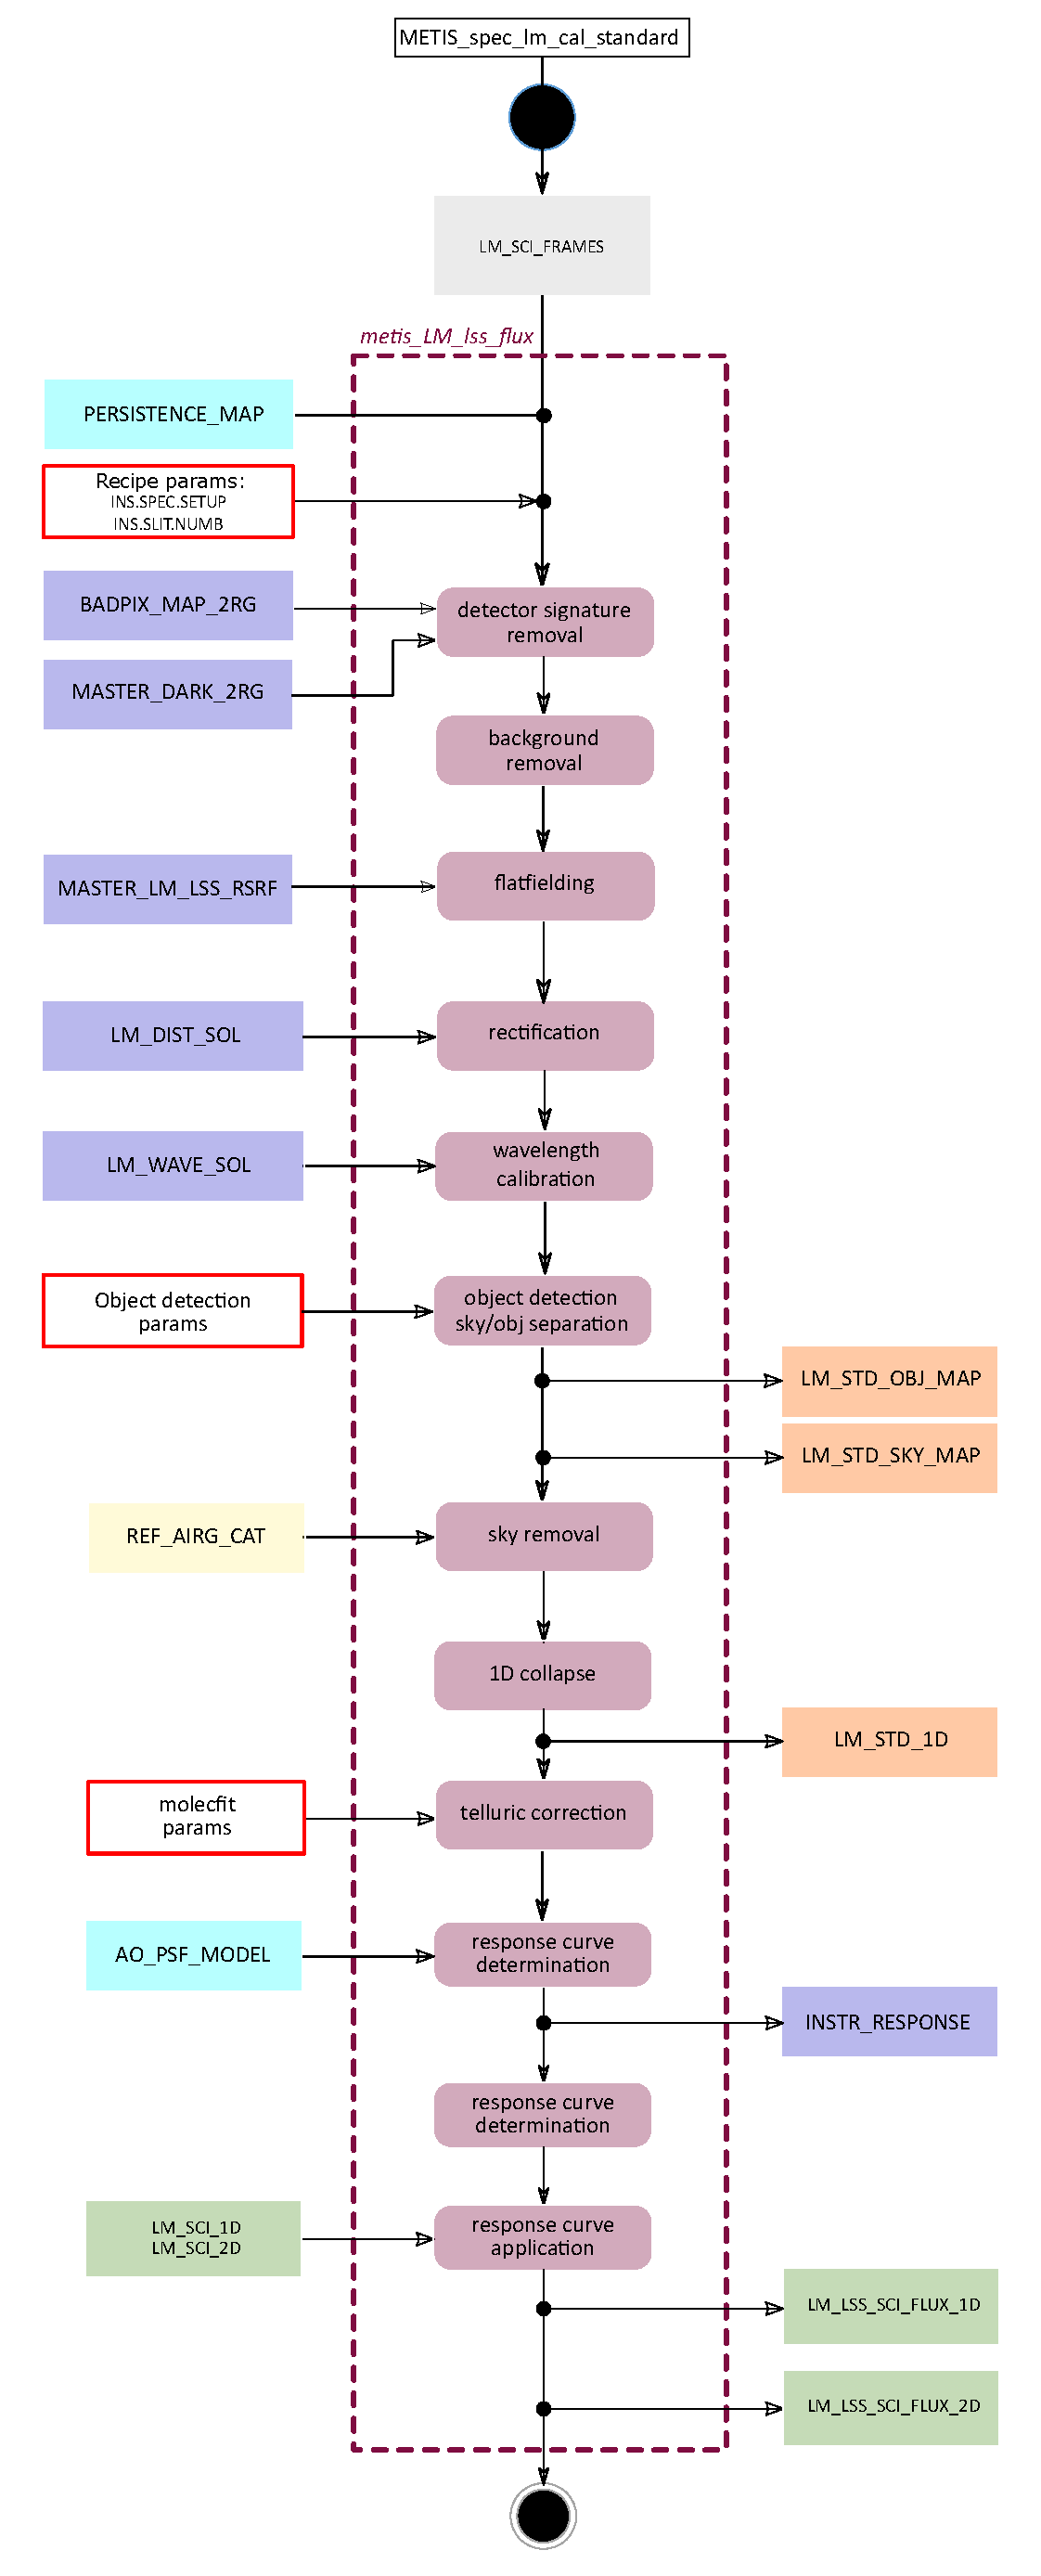
\includegraphics[width=0.4\textheight]{figures/metis_lm_lss_flux_v0.64.pdf}
  \caption[Recipe: \REC{metis_LM_lss_flux}]{\REC{metis_LM_lss_flux} --
    Flux calibration recipe.}
  \label{Fig:rec_lm_lss_flux}
\end{figure}
\clearpage
\begin{recipedef}
Name:		& \REC{metis_LM_lss_flux} \\
Purpose:	& Flux calibration \\
Type:		& Calibration\\
Requirements: & METIS-6084, METIS-6074 \\
Observing templates: & \TPL{METIS_spec_lm_acq}, \\
                & \TPL{METIS_spec_lm_obs_AutoNodOnSlit}, \\
                & \TPL{METIS_spec_lm_obs_GenericOffset} \\
                % & \TPL{METIS_spec_lm_cal_lampwave}\\
                & \TPL{METIS_spec_lm_cal_standard}\\
                & \TPL{METIS_spec_lm_cal_slit_adc}\\
Input data: 	& raw spectrophotometric STANDARD star data (\FITS{LM_FLUX_RAW})\\
                & wavelength calibrated science spectra (\PROD{LM_LSS_SCI_1D})\\
                & WCU grid for first guess distortion correction (TBD) \\
                & WCU lamp spectrum for first guess wavelength solution (TBD)\\
                & \EXTCALIB{PERSISTENCE_MAP} \\
                & \PROD{MASTER_LM_LSS_RSRF} \\
                & \PROD{MASTER_DARK_2RG} \\
                & \PROD{BADPIX_MAP_2RG} \\
                & \EXTCALIB{AO_PSF_MODEL} \\
                & \STATCALIB{ATM_LINE_CAT} \\
                % & \STATCALIB{REF_AIRG_CAT} \\
Parameters: 	& (TBD)\\
Algorithm:      & Application of master calibration files\\
                & Background removal\\
                & Determination and application of the distortion correction\\
                & Determination and application of the wavelength solution\\
                & Identifying sky/object pixels by applying e.g. Horne 1986, Ritter 2014, or by user \\
                & Removing sky lines: Creation and Subtraction of 2D sky\\
                & Collapsing 2D to 1D spectrum, (see Fig.\,\ref{Fig:rec_lm_lss_sci})\\
                & Determination and application of response curve\\
Output data:	& \PROD{LM_STD_OBJ_MAP}: Pixel map of object pixels\\
            	& \PROD{LM_STD_SKY_MAP}: Pixel map of sky pixels\\
                & \PROD{LM_STD_2D}: coadded, wavelength calibrated 2D spectrum\\
              	& \PROD{LM_STD_1D}: coadded, wavelength calibrated, collapsed 1D spectrum\\
                & \PROD{INSTR_RESPONSE}: response function (TBD)\\
                & \PROD{LM_SCI_SLIT} (\FITS{PRO_CATG=LM_LSS_2D_WAVE}): background corrected 2d spectra \\
                & \PROD{LM_SCI_OBJ_MAP}: Pixel map of object pixels\\
            	& \PROD{LM_SCI_SKY_MAP}: Pixel map of sky pixels\\
                % & \PROD{LM_SCI_2D}: coadded, wavelength calibrated 2D spectrum\\
                % & (\FITS{PRO_CATG}: \FITS{LM_LSS_2d_coadd_wavecal}) \\
                % & (\FITS{PRO_CATG}: \FITS{LM_LSS_1d_coadd_wavecal}) \\
              	& \PROD{LM_SCI_FLUX_2D}: coadded, wavelength and flux calibrated 2D spectrum\\
                & (\FITS{PRO_CATG}: \FITS{LM_LSS_2d_coadd_wavecal_flux}) \\
              	& \PROD{LM_SCI_FLUX_1D}: coadded, wavelength and flux calibrated 1D spectrum\\
                & (\FITS{PRO_CATG}: \FITS{LM_LSS_1d_coadd_wavecal_flux}) \\
                & \PROD{LM_WAVE_SOL} (\FITS{PRO.CATG=LM_WAVE_SOL}): Wavelength solution\\
                & \PROD{LM_DIST_SOL} (\FITS{PRO.CATG=LM_DIST_SOL}): Distortion solution\\
Expected accuracies: & (TBD)\\
QC1 parameters: & \QC{QC LM LSS STD BACKGD MEAN}: Mean value of background\\
                & \QC{QC LM LSS STD BACKGD MEDIAN}: Median value of background\\
                & \QC{QC LM LSS STD BACKGD SIGMA}: Sigma value of background\\
                & \QC{QC LM LSS STD SNR}: Signal-to-noise ration of flux standard star spectrum\\
                & \QC{QC LM LSS STD SNRNOISE}: Noise level of flux standard star spectrum\\
                & \QC{QC LM LSS STD FWHM}: FWHM of flux standard spectrum\\
%                & \QC{LM LSS SCI}: (TBdef) \\
                % & \QC{QC LM LSS WAVECAL DEVMEAN}: Mean deviation from the
                %   wavelength reference frame (TBDef)\\
                % & \QC{QC LM LSS WAVECAL FWHM}: Measured FWHM of lines\\
                % & \QC{QC LM LSS WAVECAL NIDENT}: Number of identified lines\\
                % & \QC{QC LM LSS WAVECAL NMATCH}: Number of lines matched between
                %     catalaogue and spectrum\\
                % & \QC{QC LM LSS WAVECAL POLYDEG}: Degree of the polynomial\\
                % & \QC{QC LM LSS WAVECAL POLYCOEFF\<n\>}: $n$-th coefficient of the polynomial\\
                & \QC{QC LM LSS FLUXCAL SNR}: Signal-to-noise ration of flux standard star spectrum\\
                & \QC{QC LM LSS FLUXCAL SNRNOISE}: Noise level of flux standard star spectrum\\
                & \QC{QC LM LSS FLUXCAL FWHM}: FWHM of flux standard spectrum\\
                & \QC{QC LM LSS FLUXCAL PSFLOSS}: percentage of AO induced slit losses (TBdef)\\
\end{recipedef}

\subsection{\REC{metis_LM_lss_sci}:}
The science calibration recipe comprises the extraction of the object (i.e. separation of object/sky pixels), removing the sky lines, the application of the response curve previously defined, the 2D to 1D collapse and the coaddition. In contrast to the flux standard star reduction, the telluric correction on the science data is done in a dedicated recipe afterwards to achieve best quality for the correction.
\begin{figure}[ht]
  \centering
  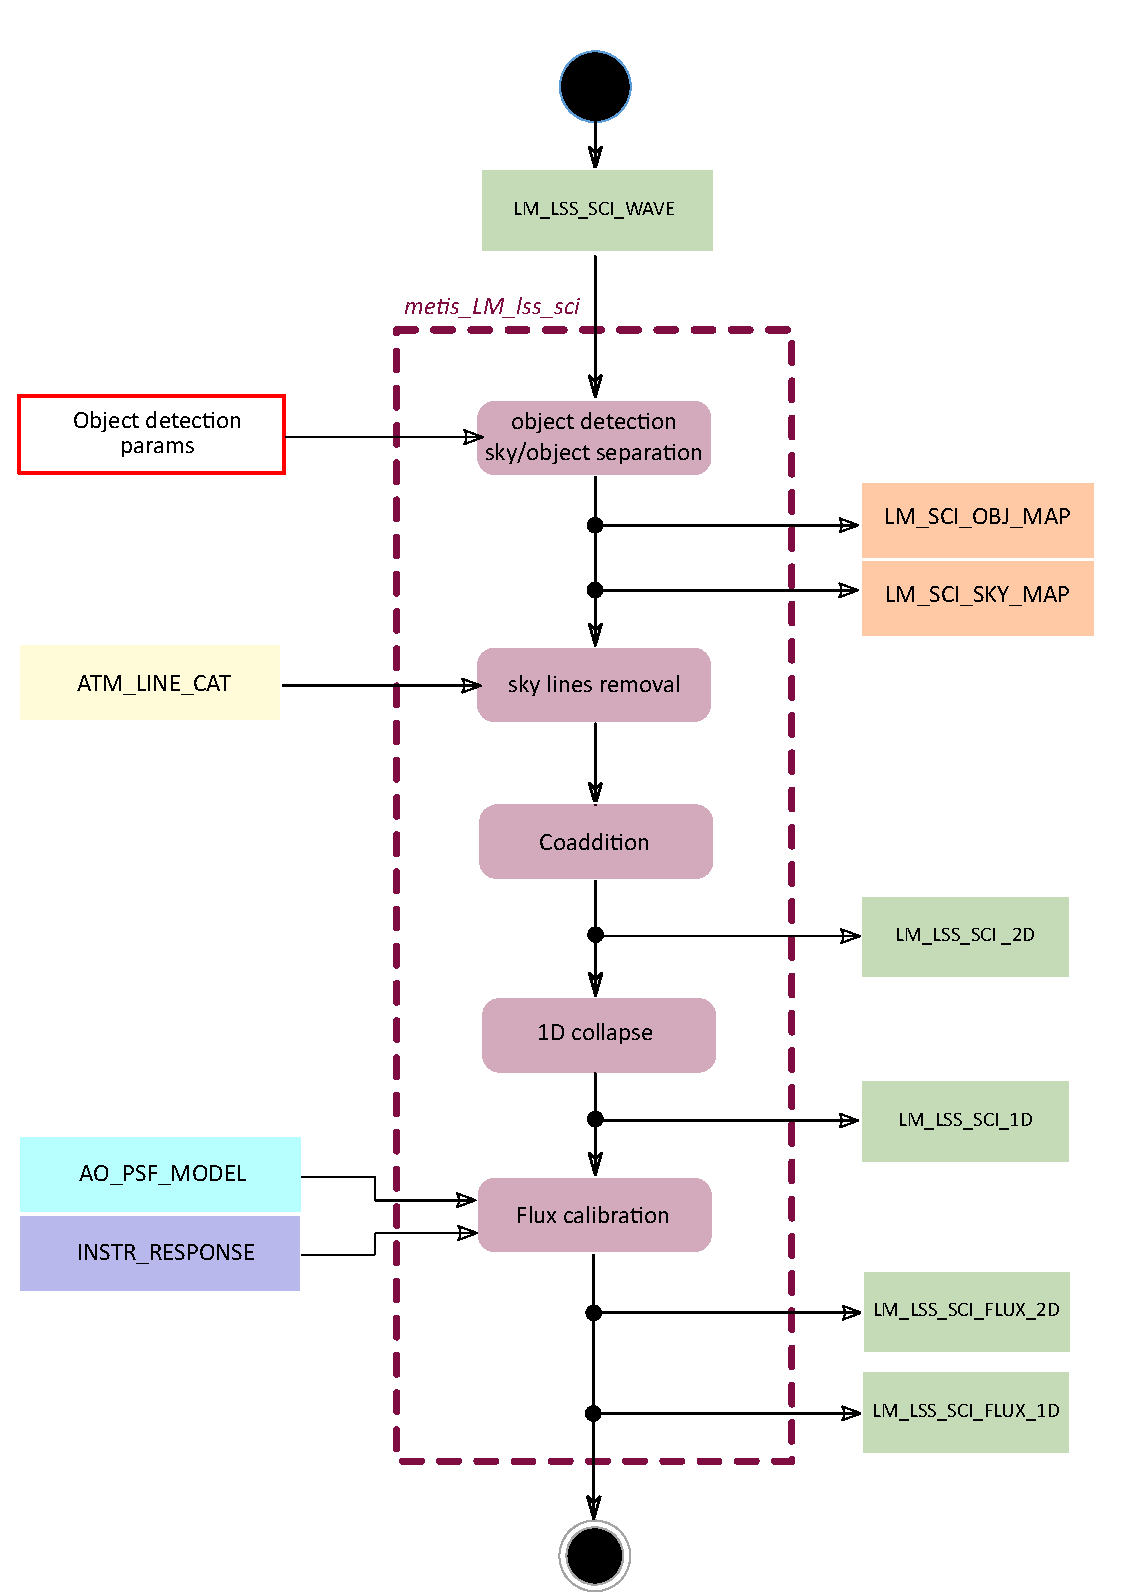
\includegraphics[width=0.5\textheight]{figures/metis_lm_lss_sci_v0.64.pdf}
  \caption[Recipe: \REC{metis_LM_lss_sci}]{\REC{metis_LM_lss_sci} --
    Science reduction recipe.}
  \label{Fig:rec_lm_lss_sci}
\end{figure}
\clearpage

\begin{recipedef}
Name:		& \REC{metis_LM_lss_sci} \\
Purpose:    Science data calibration\\
Type:		& Science reduction\\
Requirements: & METIS-6084 \\
Observing templates: & \TPL{METIS_spec_lm_acq}, \\
                & \TPL{METIS_spec_lm_obs_AutoNodOnSlit}, \\
                & \TPL{METIS_spec_lm_obs_GenericOffset} \\
                & \TPL{METIS_spec_lm_cal_slit_adc}\\
Input data: 	&  \PROD{LM_LSS_SCI_WAVE}\\
Parameters: 	& (TBD)\\
Algorithm:      & Identifying sky/object pixels by applying\\
                & Removing sky lines: Creation and Subtraction of 2D sky\\
                & Coaddition of individual object spectra of one OB\\
                & Collapsing 2D to 1D spectrum, (see Fig.\,\ref{Fig:rec_lm_lss_sci})\\
                & Application of the response function (flux calibration) \\
Output data:	& \PROD{LM_SCI_OBJ_MAP}: Pixel map of object pixels\\
            	& \PROD{LM_SCI_SKY_MAP}: Pixel map of sky pixels\\
                & \PROD{LM_LSS_SCI_2D}: coadded, wavelength calibrated 2D spectrum\\
                & (\FITS{PRO_CATG}: \FITS{LM_LSS_2d_coadd_wavecal}) \\
              	& \PROD{LM_LSS_SCI_1D}: coadded, wavelength 1D spectrum\\
                & (\FITS{PRO_CATG}: \FITS{LM_LSS_1d_coadd_wavecal}) \\
Expected accuracies: & (TBD)\\
QC1 parameters: & \QC{QC LM LSS SCI SNR}: Signal-to-noise ration of science spectrum\\
                & \QC{QC LM LSS SCI SNRNOISE}: Noise level of science spectrum\\
\end{recipedef}
